\documentclass{article}
\usepackage[utf8]{inputenc}
\usepackage[russian]{babel}
\usepackage[left=2cm,right=2cm,
top=2cm,bottom=2cm,bindingoffset=0cm]{geometry}
\usepackage{graphicx}
\usepackage{amsmath}
\usepackage{float}
\usepackage{listings}
\usepackage{url,textcomp}
\date{19 марта 2019 г.}
\author{Кондратенко Федор, гр 13632/1}
\setlength{\parindent}{0pt}
\setlength{\parskip}{5pt plus 2pt minus 1pt}
\frenchspacing
\title{Отчет по заданию №3.1}
\begin{document}
	\maketitle
	\section*{1.Теоретическая часть}
	Схема установки:
	\begin{figure}[h]
		\centering
		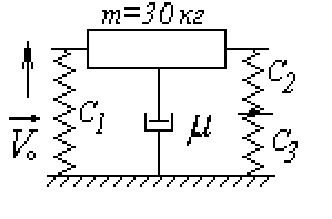
\includegraphics[width=0.3\linewidth]{C:/MATLAB/3.1/schem3}
		\caption{Схема установки}

	\end{figure}
	~\\
	~\\\\
	Исходные данные:
	$V_0=3.5$ м/с,
	$C_1=2.25$ Кн/м,
	$C_2=4$ Кн/м,
	$C_3=6$ Кн/м.
	$b=1200$ Нс/м.
	~\\
	Эквивалентая жесткость пружины:
	$$C=\frac{C_2*C_3}{C_2+C_3}+C_1=4650$$
	Дифференциальное уравнение колебания груза без учета сил трения и без воздействия на него внешних сил имеет вид:
	$$mx''+cx=0$$
	С трением:
	$$mx''+bx'+cx=0$$
	Собственная частота системы:
	$$k=\sqrt{\frac{c}{m}}=12.44989$$
	Блок-схема вычисления собственной частоты модели:
	\begin{figure}
		\centering
		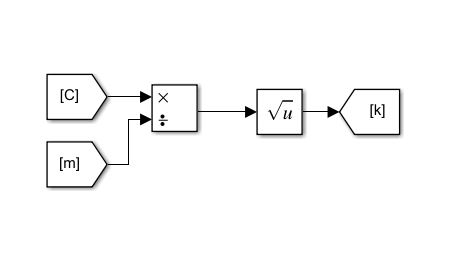
\includegraphics[width=0.7\linewidth]{schem5}
		\caption{Блок-схема вычисления собственной частоты}

	\end{figure}
	Период колебаний груза без учета трения:
	$$T=\frac{2\pi}{k}=0.5047$$
	Собственная частота колебани с учетом трения:
	$$k_1=\sqrt{k^2-(\frac{b}{2m})^2}$$
	Для указанных в задании параметров невозможно расчитать частоту колебаний с учетом демпфирования, поскольку подкоренное выражение отрицательно. 
	\section*{2.Моделирование колебаний груза без трения}
	Уравнение:
	$$x''=-\frac{c}{m}x$$
	Блок-схема:
	\begin{figure}[h!]
		\centering
		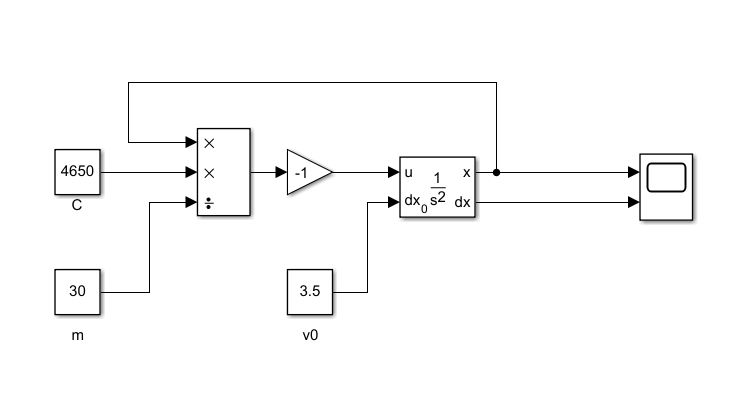
\includegraphics[width=0.7\linewidth]{C:/MATLAB/3.1/schem1}
		\caption{Блок-схема}

	\end{figure}
	~\\
	~\\\\
	~\\
	~\\\\
	~\\
	~\\\\~\\
	~\\\\
	График колебаний:
	\begin{figure}[H]
		\centering
		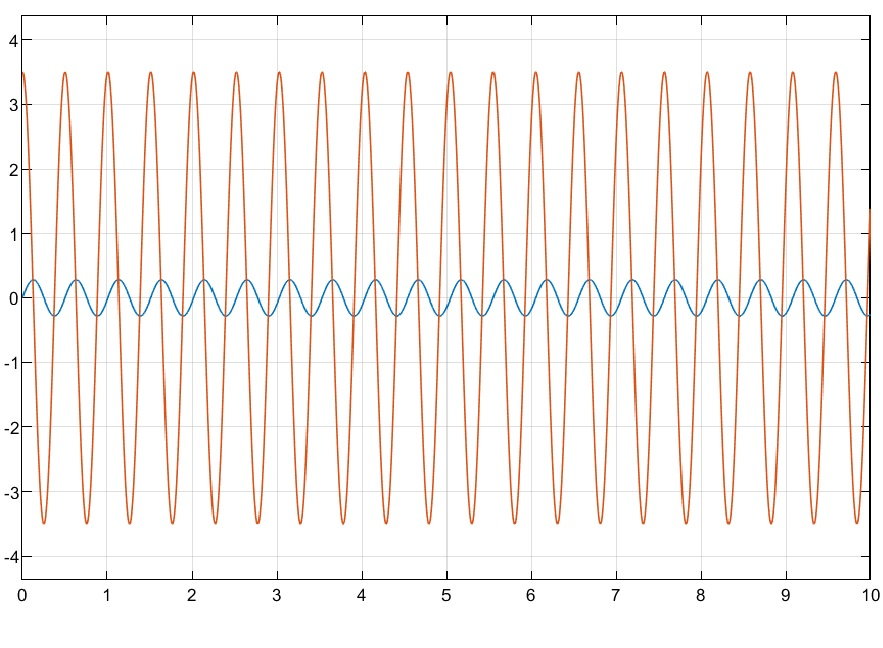
\includegraphics[width=0.7\linewidth]{C:/MATLAB/3.1/graph1}
		\caption{График координат и скорости груза}

	\end{figure}
	
	
	\section*{3. Моделирование колебаний груза с учетом вязкого трения}
	Дифференциальное уравнение колебаний при наличии вязкого трения:

	$$x''=-\frac{1}{m}(bx'+cx)$$
	Блок-схема:
	\begin{figure}[H]
		\centering
		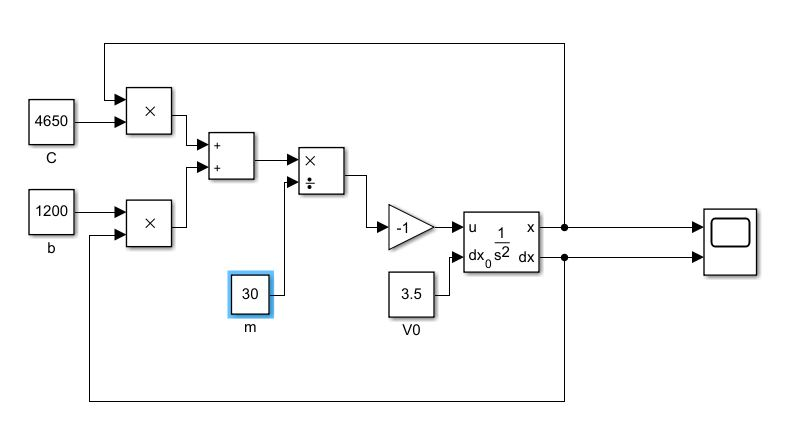
\includegraphics[width=0.6\linewidth]{C:/MATLAB/3.1/schem2}
		\caption{Блок-схема для модеkирования колебаний с учетом вязкого трения}

	\end{figure}
	График колебаний груза:
	\begin{figure}[H]
		\centering
		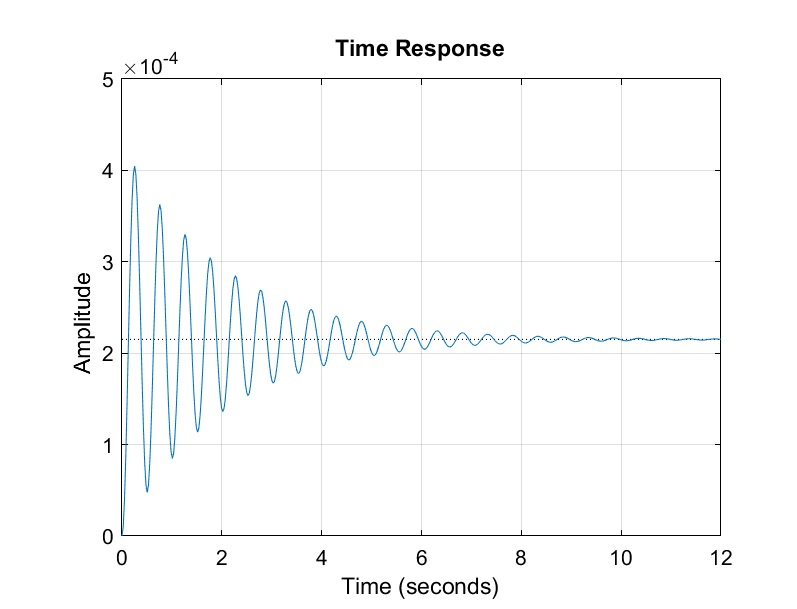
\includegraphics[width=0.7\linewidth]{C:/MATLAB/3.1/graph2}
		\caption{Колебания груза с учетом трения}

	\end{figure}
	Как можно видеть из графика, колебаний груза не происходит.
	Колебание с отрицательным демпифрованием:
	\begin{figure}[H]
		\centering
		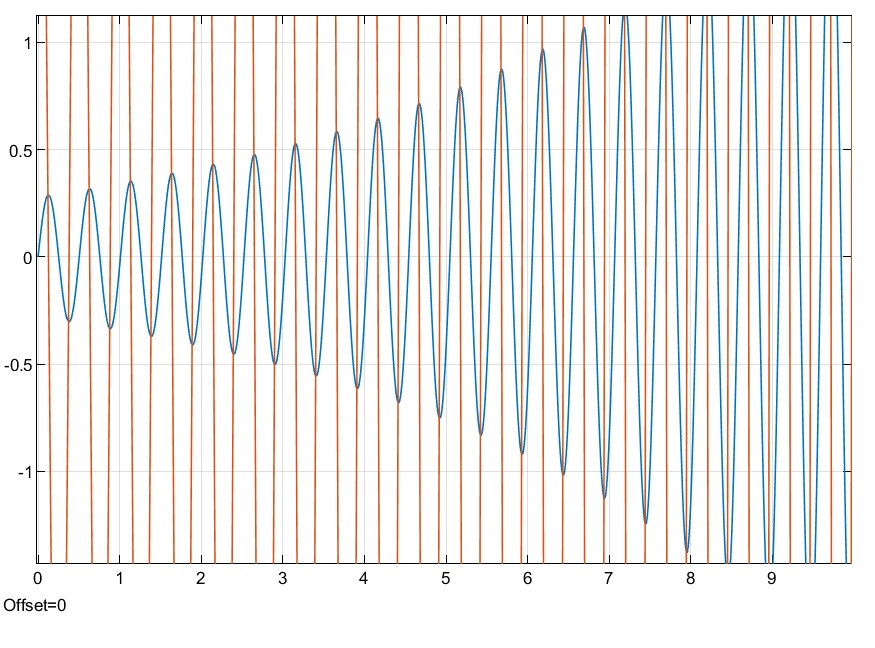
\includegraphics[width=0.7\linewidth]{graph4}
		\caption{График колебаний с отрицательным демпфированием}

	\end{figure}
	Из графика видно, что амплитуда экспоненциально растет.
	
	\section*{Резонанс, биение, бигармонический процесс}
	Резонанс без сопротивления:
	\begin{figure}[H]
		\centering
		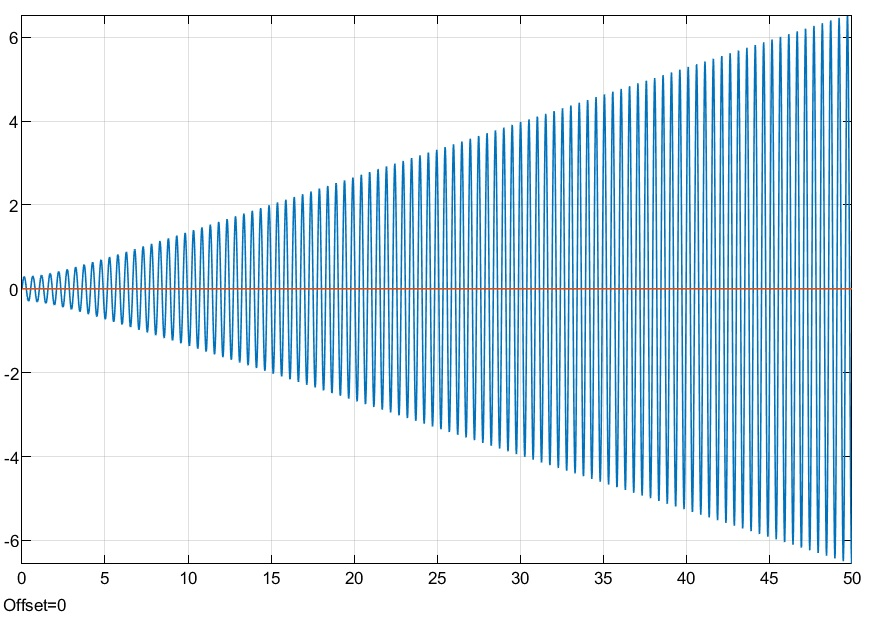
\includegraphics[width=0.7\linewidth]{graph8}
		\caption{Резонанс без сопротивления, $\omega = k = 12.45$}

	\end{figure}
	Как видно из графика, амплитуда линейно растет.
	Резонанс с сопротивлением удалось получить только при уменьшении коэффициента демпфирования:
	\begin{figure}[H]
		\centering
		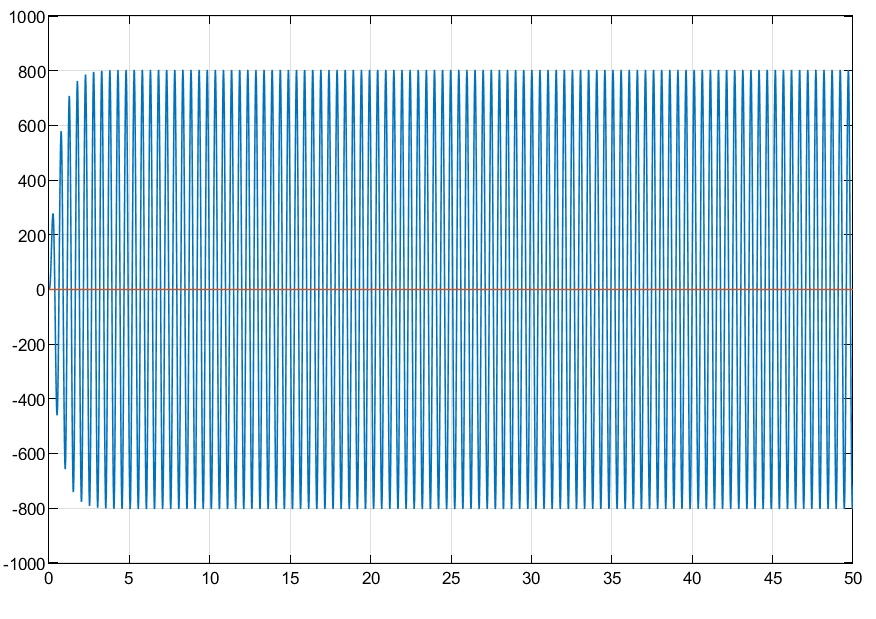
\includegraphics[width=0.7\linewidth]{graph10}
		\caption{Резонанс с сопротивлением, коэффициент демпфирования уменьшен до $b=100, \omega = k = 12.45$}

	\end{figure}
	Биение без сопротивления. Амплитуда изменяется по гармоническому закону:
	\begin{figure}[H]
		\centering
		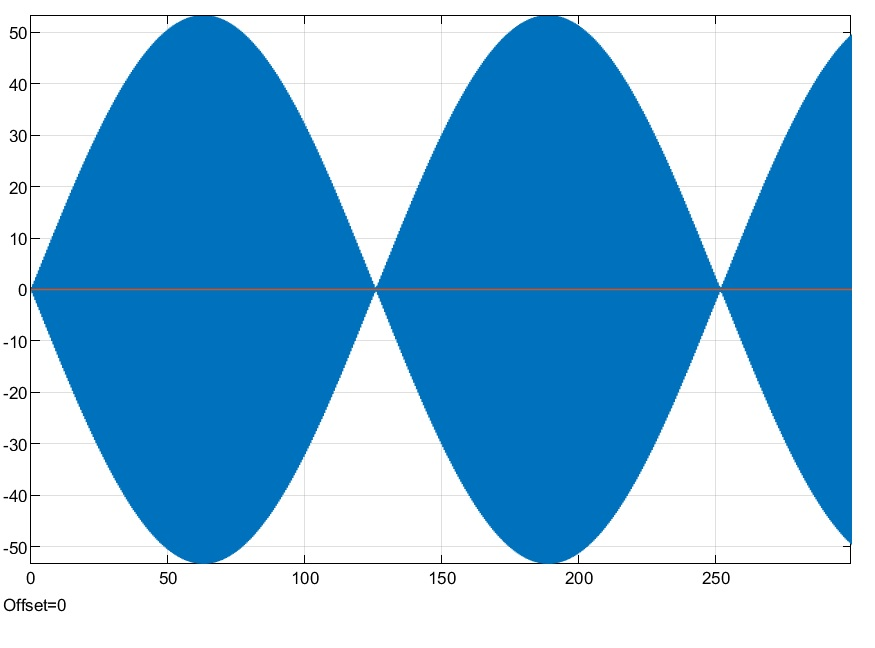
\includegraphics[width=0.7\linewidth]{graph5}
		\caption{Биение без сопротивления $b=0, k = 12.45, \omega = 12.3$}

	\end{figure}
	Биение с сопротивлением удалось получить при очень маленьком коэффициенте демпфирования:
	\begin{figure}[H]
		\centering
		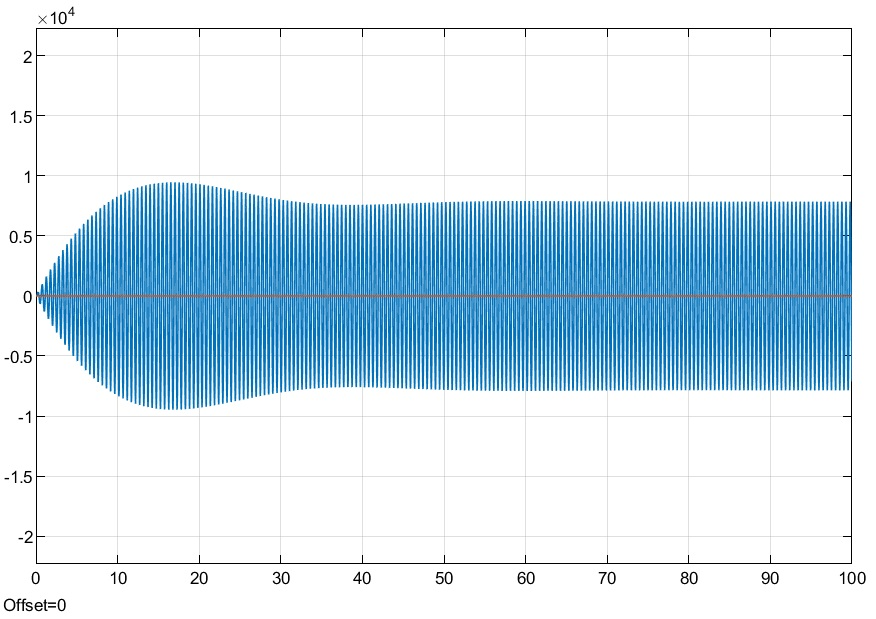
\includegraphics[width=0.7\linewidth]{graph11}
		\caption{Биение с сопротивлением, коэффициент демпфирования $b=5, k = 12.45, \omega = 12.3$}

	\end{figure}
	
	Бигармонический процесс без сопротивления:
	\begin{figure}[H]
		\centering
		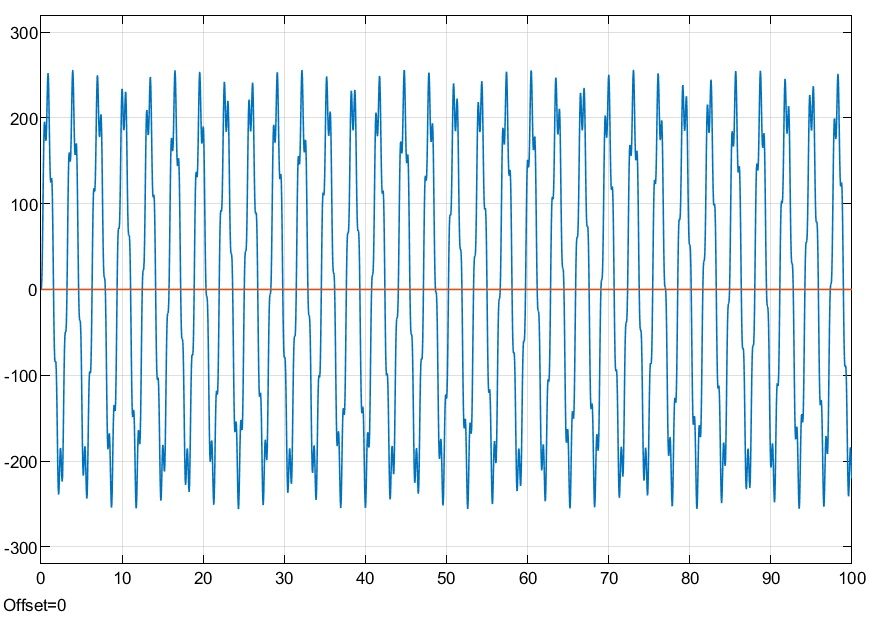
\includegraphics[width=0.7\linewidth]{graph9}
		\caption{Бигармонический процесс без сопротивления, $b = 0, \omega = 2, k = 12.45$}
	\end{figure}
	Бигармонический процесс с сопротивлением:
	\begin{figure}[H]
		\centering
		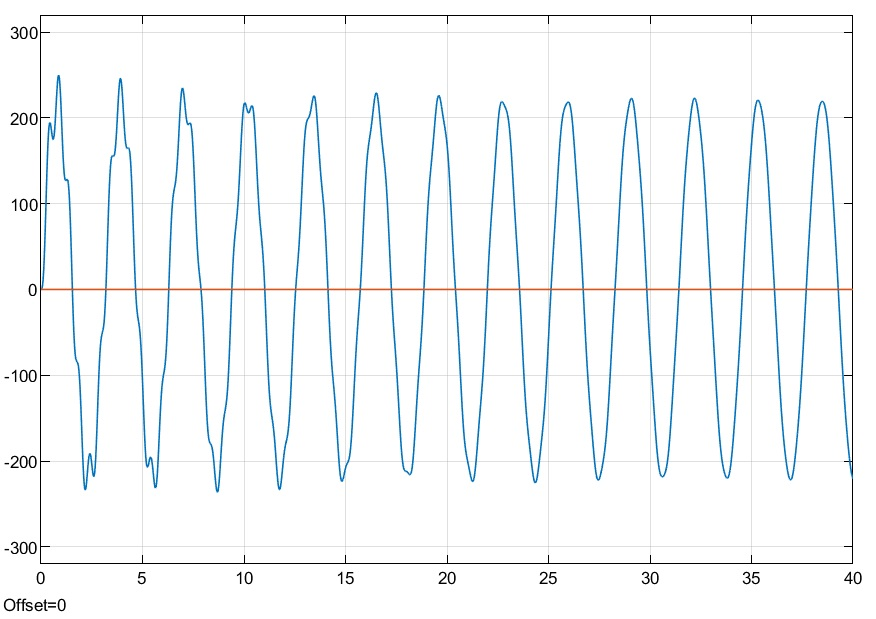
\includegraphics[width=0.7\linewidth]{graph12}
		\caption{Бигармонический процесс с сопротивлением, $b = 5, \omega = 2, k = 12.45$}
	\end{figure}
	На графике отчетливво виден период в 20-25 секунд, в течение которого бигармоничекий процесс прекращается, остаются лишь вынужденные колебания.
	
	Итоговая схема, использованная для моделирования:
	\begin{figure}[H]
		\centering
		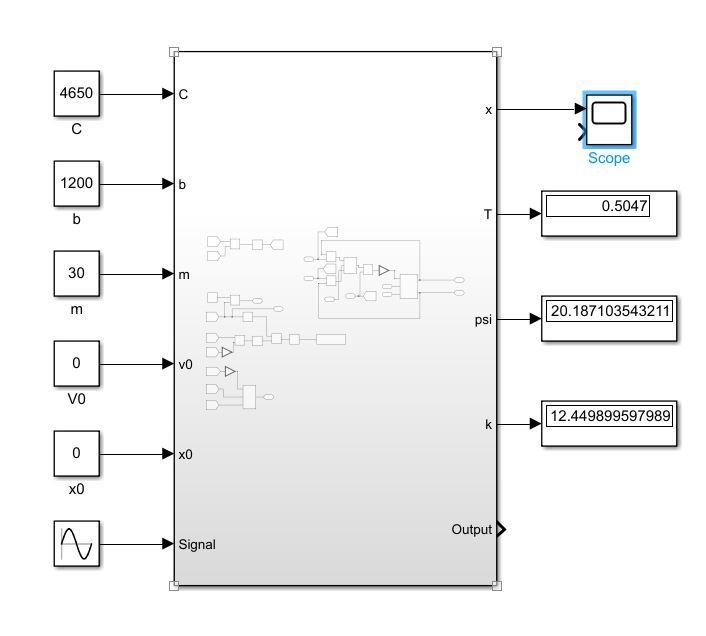
\includegraphics[width=0.7\linewidth]{schem4}
		\caption{Блок-схема модели}

	\end{figure}
	Блок-схема подсистемы:
	\begin{figure}[H]
		\centering
		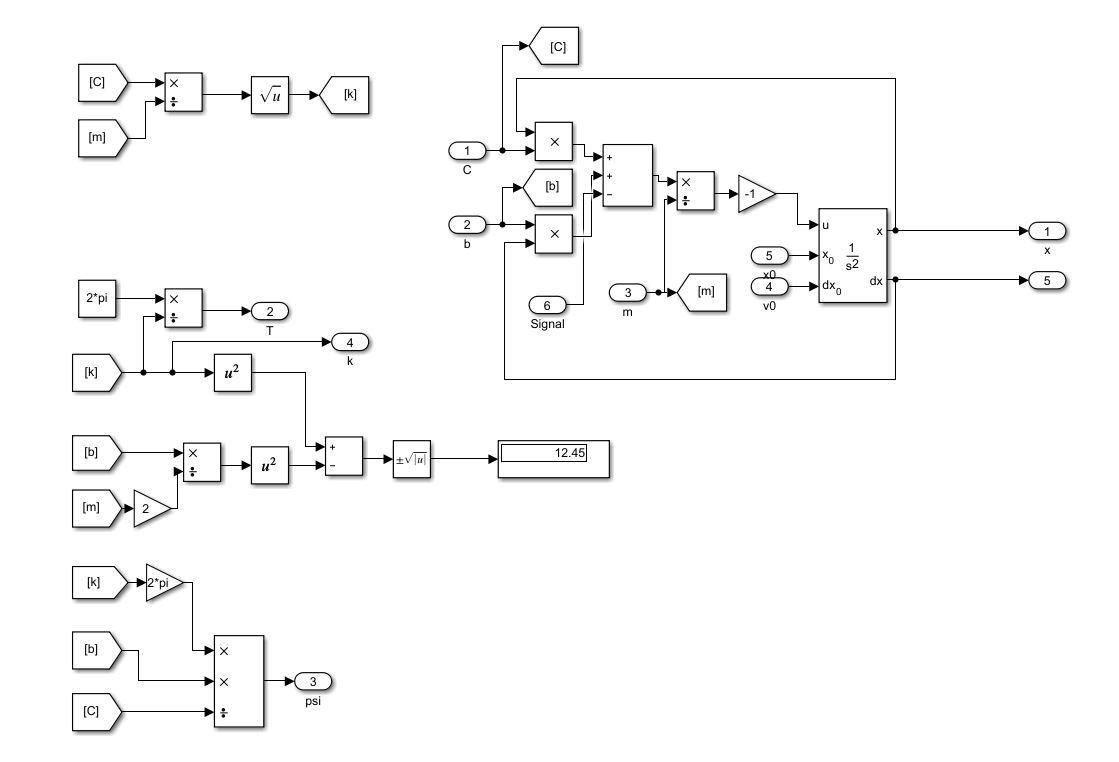
\includegraphics[width=0.7\linewidth]{schem6}
		\caption{Подсистема модели}
	\end{figure}
	


	
\end{document}